\documentclass[a0,portrait]{a0poster}

\usepackage{multicol}
\columnsep=100pt 
\columnseprule=5pt 

\usepackage[svgnames]{xcolor}
\usepackage{times} 
\usepackage{graphicx} 
\graphicspath{{figures/}} 
\usepackage{booktabs} 
\usepackage[font=small,labelfont=bf]{caption} 
\usepackage{amsfonts, amsmath, amsthm, amssymb} 
\usepackage{wrapfig}

\begin{document}
\begin{minipage}[b]{0.8\linewidth}
\color{NavyBlue} \VeryHuge{\textbf{Digitalne urbane mreže i društveni mediji}} 
\color{Black}\\

\huge \textbf{Tamara Jevtimijević, 261/2017}\\[0.5cm]
\huge Računarstvo i društvo, Matematički fakultet u Beogradu\\[0.4cm] 
\Large \textit{mi17261@alas.matf.bg.ac.rs}\\
\end{minipage}
\begin{minipage}[b]{0.2\linewidth}

\includegraphics[width=12cm]{logo.png}\\
\end{minipage}
\vspace{3cm} 
\begin{multicols}{2} 
\color{Black}
\color{Black}
\section*{}
\Large{
Krajem XX i početkom XXI veka informaciono - komunikacione \\ korporacije su doživele najveću ekspanziju. Danas ih ima sve više i sve su uticajnije. Tehnologije su uznapredovale velikom brzinom i svoje grane su pustile svuda. Danas gde god da se okrenemo digitalizacija je oko nas. 
}

\color{teal}

\vspace{100}
\section*{\huge{\textit{Teme:}}}

\begin{enumerate}
\item \textit{Statistike napredovanja pametnih gradova kroz monopol.}
\item \textit{Rešavanje problema stranih start - apova.}
\item \textit{Digitalna urbana infrastruktura.}
\item \textit{Uspon informaciono - komunikacionih tehnologija.}
\item \textit{Monopol IKT-a.}
\item \textit{Društvene mreže i grad.}
\item \textit{Urbano brendiranje i društvene mreže.}
\end{enumerate}

\color{black}

\vspace{100}
\section*{\Huge{Društvene mreže i grad}}

\Large{
Uspon društvenih mreža kao što su Facebook, Twitter, WeChat, Tumblr, Instagram, Google+, YouTube, Linkedin, TikTok, Snapchat i WhatsApp promenio je način na koji ljudi širom sveta komuniciraju i žive. Čini se da ljudi više vole i primenjuju digitalne interakcije u odnosu na fizičke interakcije. 
Procenjuje se da preko 3,2 milijarde ljudi širom sveta koristite društvene mreže na ovaj ili onaj način, a ovi trendovi su zaslužni za širok prodor pametnih telefona i tableta.
}

\begin{center}\vspace{2cm}
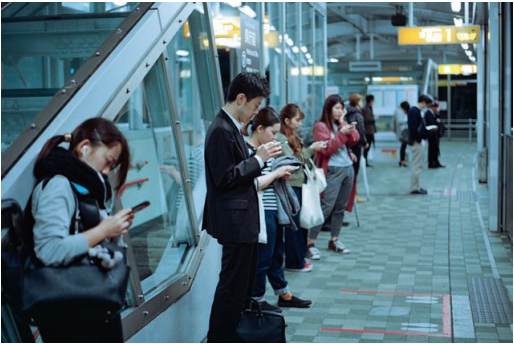
\includegraphics[width=35cm,height=25cm]{mreze.png}
\end{center}\vspace{12cm}

\section*{\Huge{Urbano brendiranje i društvene mreže}}

\Large{
Digitalni brend je dao gradovima priliku da digitalne tehnologije iskoriste na ekonomskom području. Nakon pojave društvenih mreža, turistički brendovi su prihvaćeni u različitim gradovima. Brendiranje je strategija koja je usvojena, da bi se oni, koji žive u nekom gradu, ali i oni koji su samo njegovi posetioci osetili njegovim delom.
}

\begin{center}\vspace{1cm}
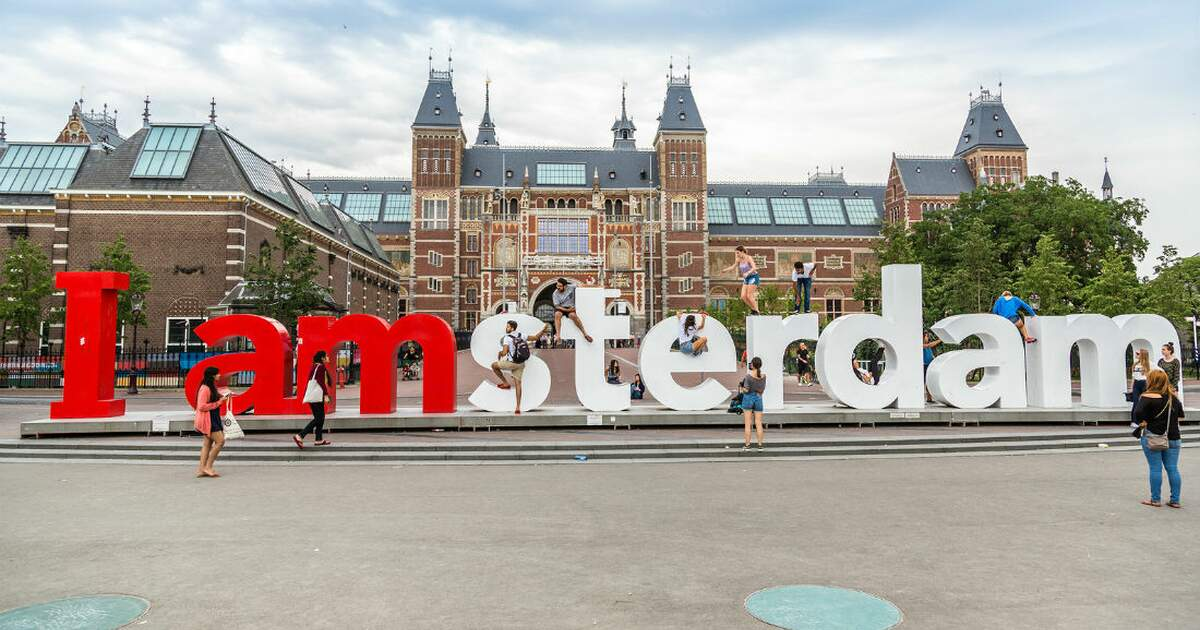
\includegraphics[width=30cm,height=20cm]{rijksmuseum-amsterdam-museum-iamsterdam.jpg}
\end{center}\vspace{1cm}

\begin{center}\vspace{1cm}

\includegraphics[width=30cm,height=25cm]{Quinonez_Julian_Istanbul_Logo.png}
\end{center}\vspace{1cm}


\color{SaddleBrown} % SaddleBrown color for the conclusions to make them stand out

\color{teal}

\section*{\huge{Zaključak}}

\Large{
Možemo primetiti sve veću ulogu digitalnih medija u
oblikovanju gradske privrede i političke sfere. Uloga društvenih medija, odnosno mreža u gradovima, posebno u javnim prostorima, postaje sve više naglašena. Vidi se i da političari sve više koriste društvene platforme, kako bi stekli političku kilometražu i ekonomsku otpornost.
}

\end{multicols}
\end{document}